\documentclass[10pt]{article}

% Pacotes extras necessários
\usepackage{amsmath}
\usepackage[lmargin=0.5in, rmargin=0.5in, tmargin=0.5in, bmargin=0.5in, includehead, includefoot]{geometry}
\usepackage{amsfonts}
\usepackage[utf8]{inputenc}
\usepackage[portuguese]{babel}
\usepackage{graphicx}
\usepackage{fancyhdr}
\usepackage{setspace}

\graphicspath{ {./images/} }

% Sets para outras partes
\setlength{\parindent}{0pt}
\setstretch{1.5}
\DeclareMathOperator{\sen}{sen}
\DeclareMathOperator{\sinc}{sinc}

%% Facilidades
%% -- Laplace
\newcommand{\Lap}[1]{\mathcal{L}\left\{#1\right\}}

%% -- Fourier
\newcommand{\Fou}[1]{\mathcal{F}\left\{#1\right\}}

%% -- Transformada Z
\newcommand{\Z}[1]{\mathcal{Z}\left\{#1\right\}}

%% -- Negrito em matemáticas
\newcommand{\bm}[1]{\boldsymbol{#1}}


% ------- Estilo do trabalho -------- %
\fancypagestyle{capa}{
    \fancyhf{}
    \renewcommand\headrulewidth{0pt}
    \fancyfoot[C]{
        Rio de Janeiro\\
        2022
    }
}

\pagestyle{fancy}
\fancyhead{}
\fancyhead[L]{\thepage}
\fancyfoot{}
% ----------------------------------- %

% Dados do Grupo
\title{Sinais e Sistemas - Trabalho 6 - Avaliação 10}
\author{
    \textbf{Grupo 2}\\
    Leonardo Soares da Costa Tanaka\\
    Matheus Henrique Sant Anna Cardoso\\
    Theo Rudra Macedo e Silva
}
\date{}

\begin{document}
\maketitle
\thispagestyle{capa}
\newpage

\textbf{1.)} Considere o sinal $v(t) = e^{-2t^2}$. (\textbf{Grupo 2:})

(a) Plote o seu gráfico;

\begin{verbatim}
%Questão 1.a)

% Intervalo
dt=0.001;

% Dados basicos
t=-2:dt:2-dt;
v=exp(-2*t.^2);
plot (t, v, "r", "linewidth", 3);
title("v(t) por t - 1.a)", "fontsize", 20);
xlabel("t", "fontsize", 18);
ylabel("v(t)", "fontsize", 18);
\end{verbatim}

\begin{figure}[h]
    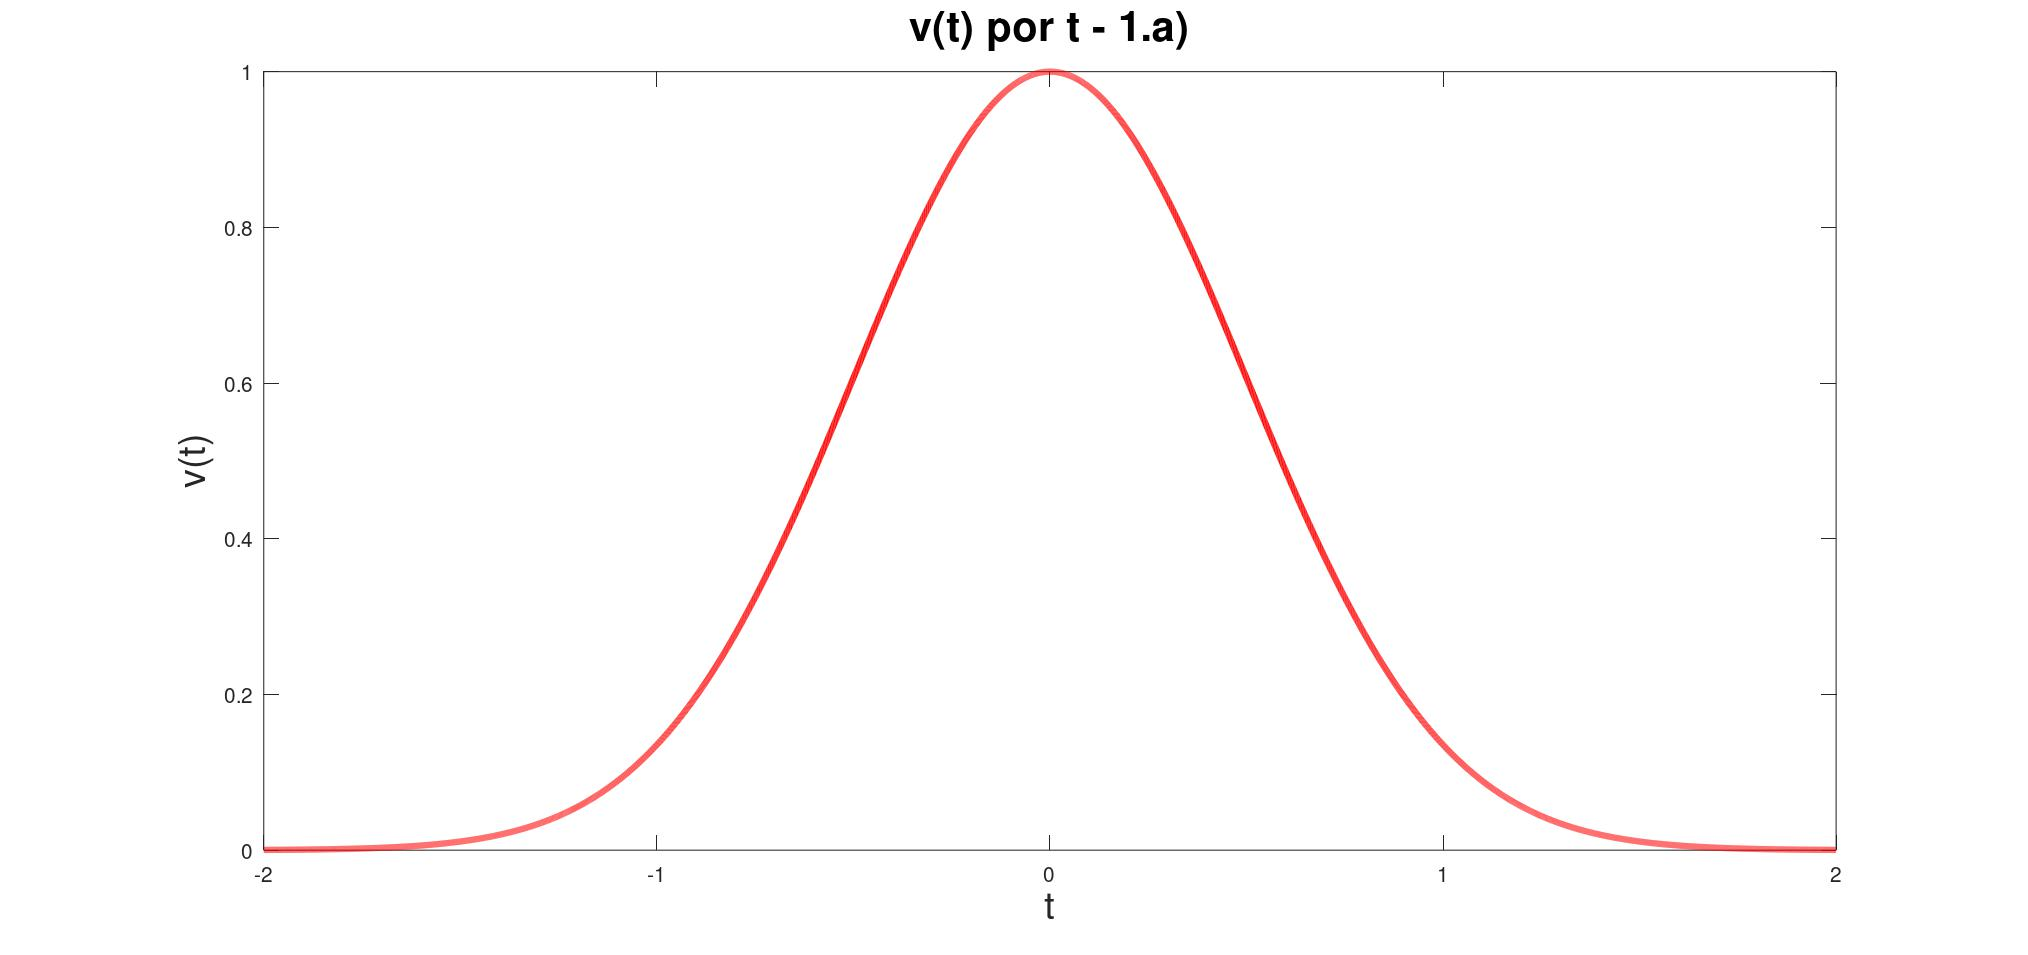
\includegraphics[scale=0.2]{questao1a}
    \centering
\end{figure}

(b) escolha, a seu critério, uma janela de amostragem apropriada;

\vspace{\baselineskip}
Foi escolhida uma janela de amostragem de 4 de largura com começo em -2, porque foi quando a função v começa a ficar maior que zero e depois começa a voltar para o zero.
\vspace{\baselineskip}

(c) escolha uma frequência de amostragem $f_a$ bem pequena, que coloque poucos pontos na janela, ache a FFt da série temporal obtida e analise o espectro de magnigudes;

\vspace{\baselineskip}
Foi escolhida uma frequência de amostragem $f_a$ de 1/$\Delta_T$ que nesse caso seria 2,5.

\begin{verbatim}
    dt=0.4;
    t=-2:dt:2;
    v=exp(-2*t.^2);
    plot (t, v, "r*-", "linewidth", 3);
    title("v(t) por t - 1.c)", "fontsize", 20);
    xlabel("t", "fontsize", 18);
    ylabel("v(t)", "fontsize", 18);
\end{verbatim}

\begin{figure}[h]
    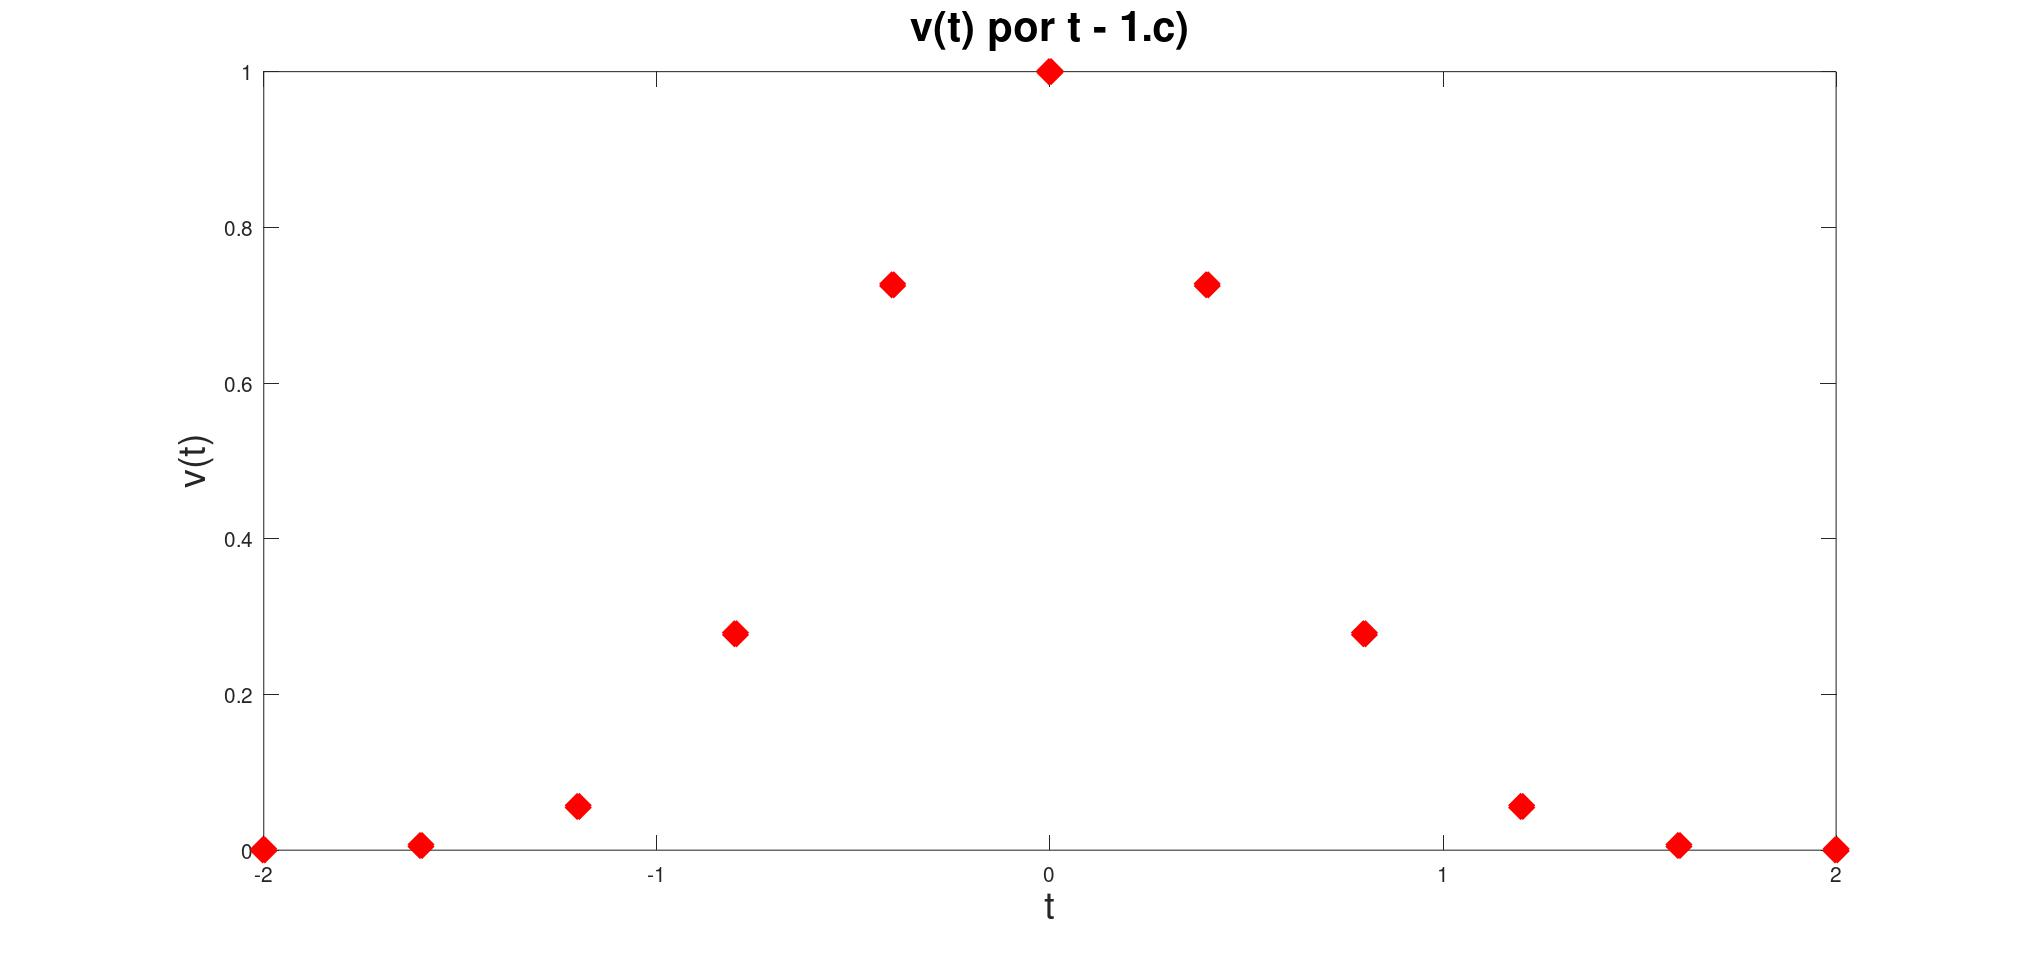
\includegraphics[scale=0.2]{questao1c}
    \centering
\end{figure}

Então é preciso fazer as seguintes operações para calcular a FFT:

$\Delta_f = 1/T_0 = 1/4 = 0.25; \ L_0 = (N - 1)\Delta_f = 2,5 \Rightarrow f \in [-1,25 \ 1,25]$

\begin{verbatim}
f=-1.25:(0.25):1.25;
V = fft(v)
V = fftshift(V);
modV = abs(V);
plot(f, modV, "r*-", "linewidth", 3)
title("Espectro de magnitudes", "fontsize", 20);
\end{verbatim}

\begin{align*}
    FFT: \\
    3.1333 +      0i \\
    -2.3299 - 0.6841i \\
    0.9509 + 0.6111i \\
    -0.2069 - 0.2388i \\
    0.0220 + 0.04
\end{align*}

\begin{figure}[h]
    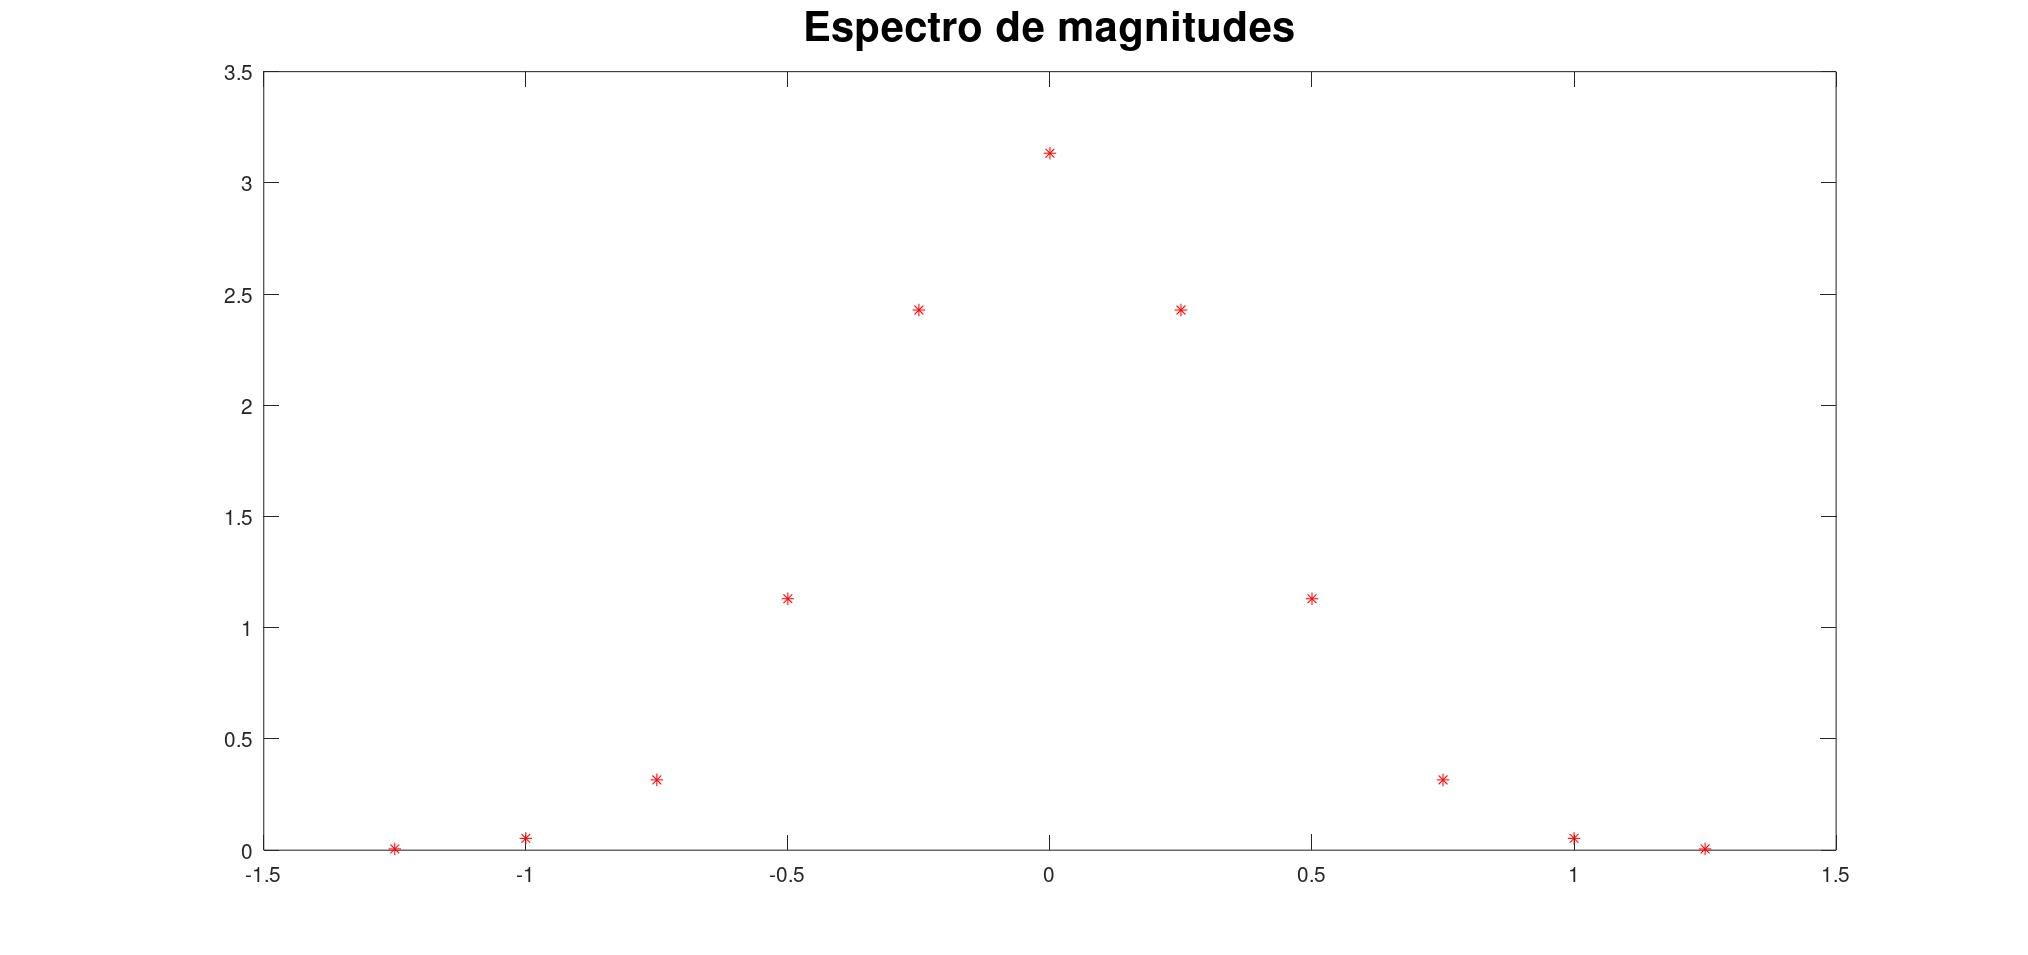
\includegraphics[scale=0.2]{questao1c2}
    \centering
\end{figure}

(d) escolha a $f_a$ maior que a anterior, que coloque mais pontos na janela, ache a FFT correspondente e compare com a anterior;

\begin{verbatim}
dt=0.2;
t=-2:dt:2;
v=exp(-2*t.^2);
plot (t, v, "rx", "linewidth", 10);
title("v(t) por t - 1.d)", "fontsize", 20);
xlabel("t", "fontsize", 18);
ylabel("v(t)", "fontsize", 18);   
\end{verbatim}

\begin{figure}[h]
    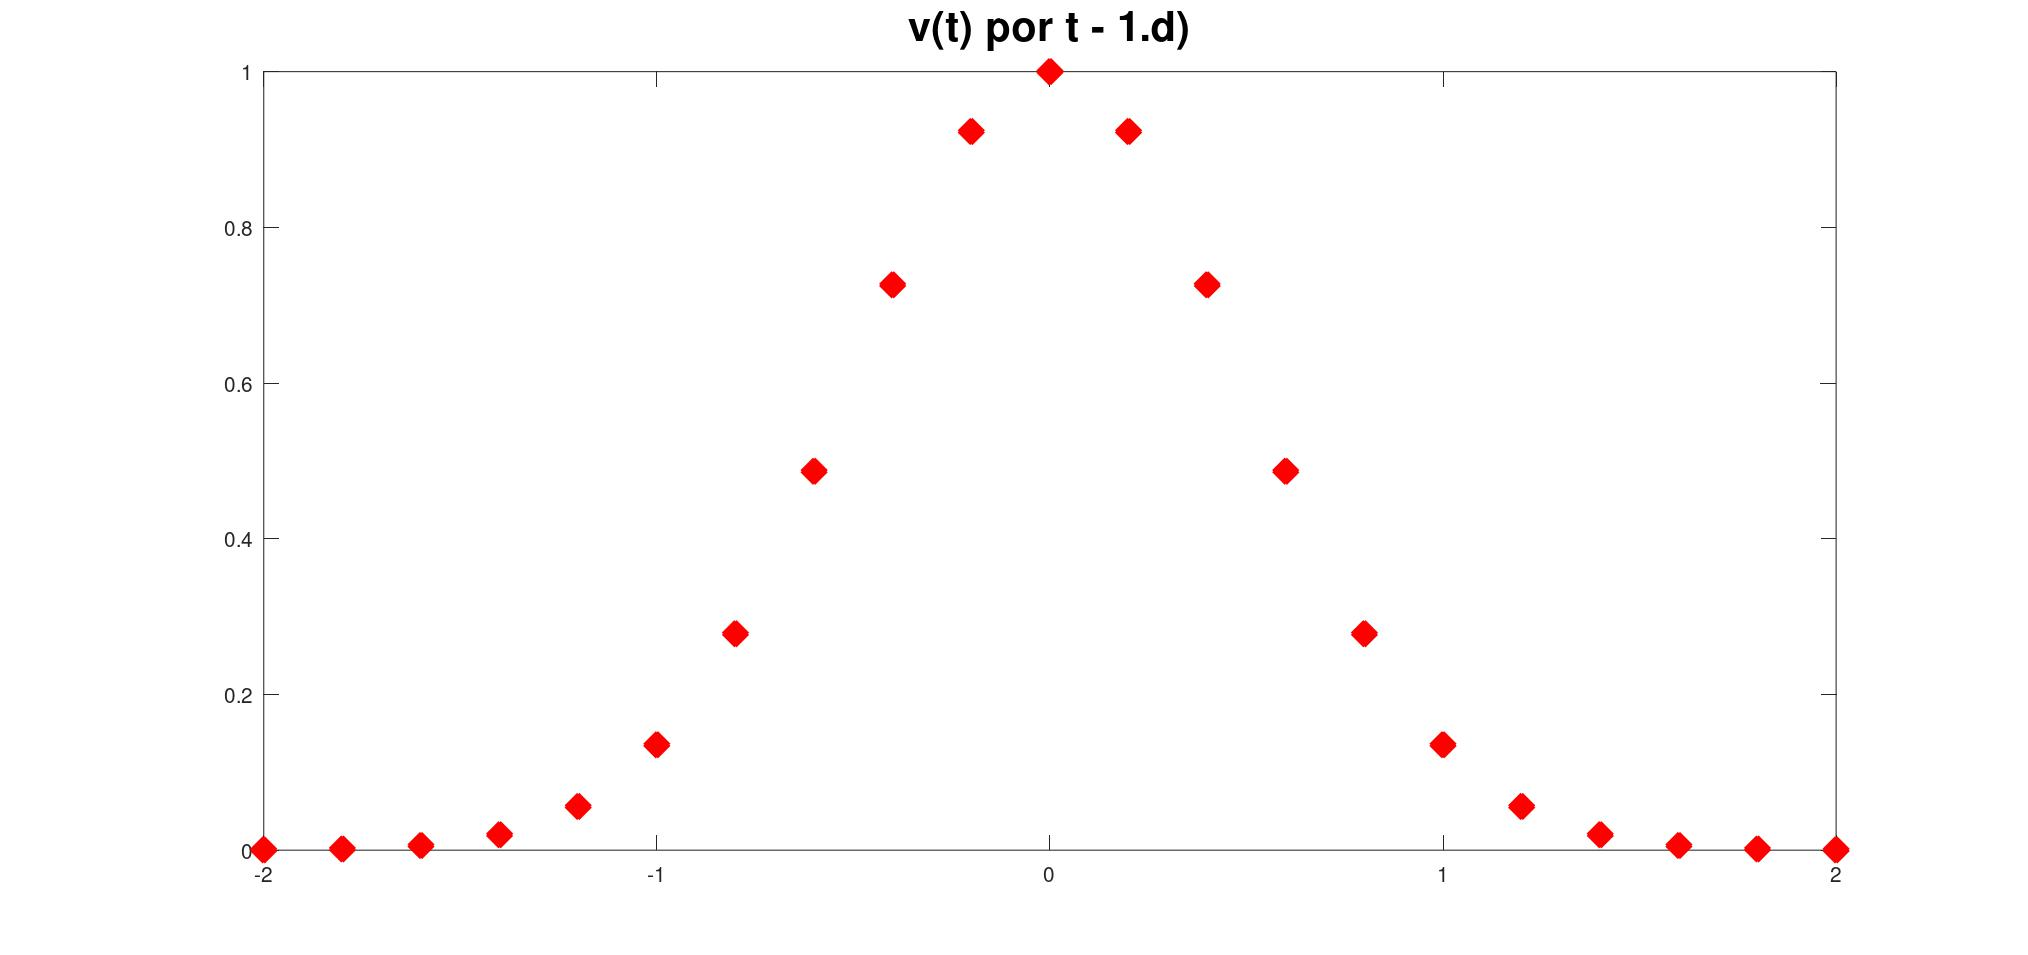
\includegraphics[scale=0.2]{questao1d}
    \centering
\end{figure}

$\Delta_f = 1/T_0 = 1/4 = 0.25; \ L_0 = (N - 1)\Delta_f = 5 \Rightarrow f \in [-2,5 \ 2,5]$

\begin{verbatim}
f=-2.5:(0.25):2.5;
V = fft(v)
V = fftshift(V);
modV = abs(V);
plot(f, modV, "r*")
title("Espectro de magnitudes", "fontsize", 20); 
\end{verbatim}

\begin{align*}
    && && FFT: \\
    6.2664 +      0i && -4.6846 - 0.7061i &&  1.9556 + 0.6032i && -0.4554 - 0.2193i &&  0.0588 + 0.0401i \\
   -0.0043 - 0.0040i &&  0.0001 + 0.0002i && -0.0000 - 0.0000i && -0.0000 - 0.0000i && -0.0000 - 0.0000i \\
   -0.0000 - 0.0000i && -0.0000 + 0.0000i && -0.0000 + 0.0000i && -0.0000 + 0.0000i && -0.0000 + 0.0000i \\
    0.0001 - 0.0002i && -0.0043 + 0.0040i &&  0.0588 - 0.0401i && -0.4554 + 0.2193i && 1.9556 - 0.6032i \\
   -4.6846 + 0.7061i
\end{align*}

\begin{figure}[h]
    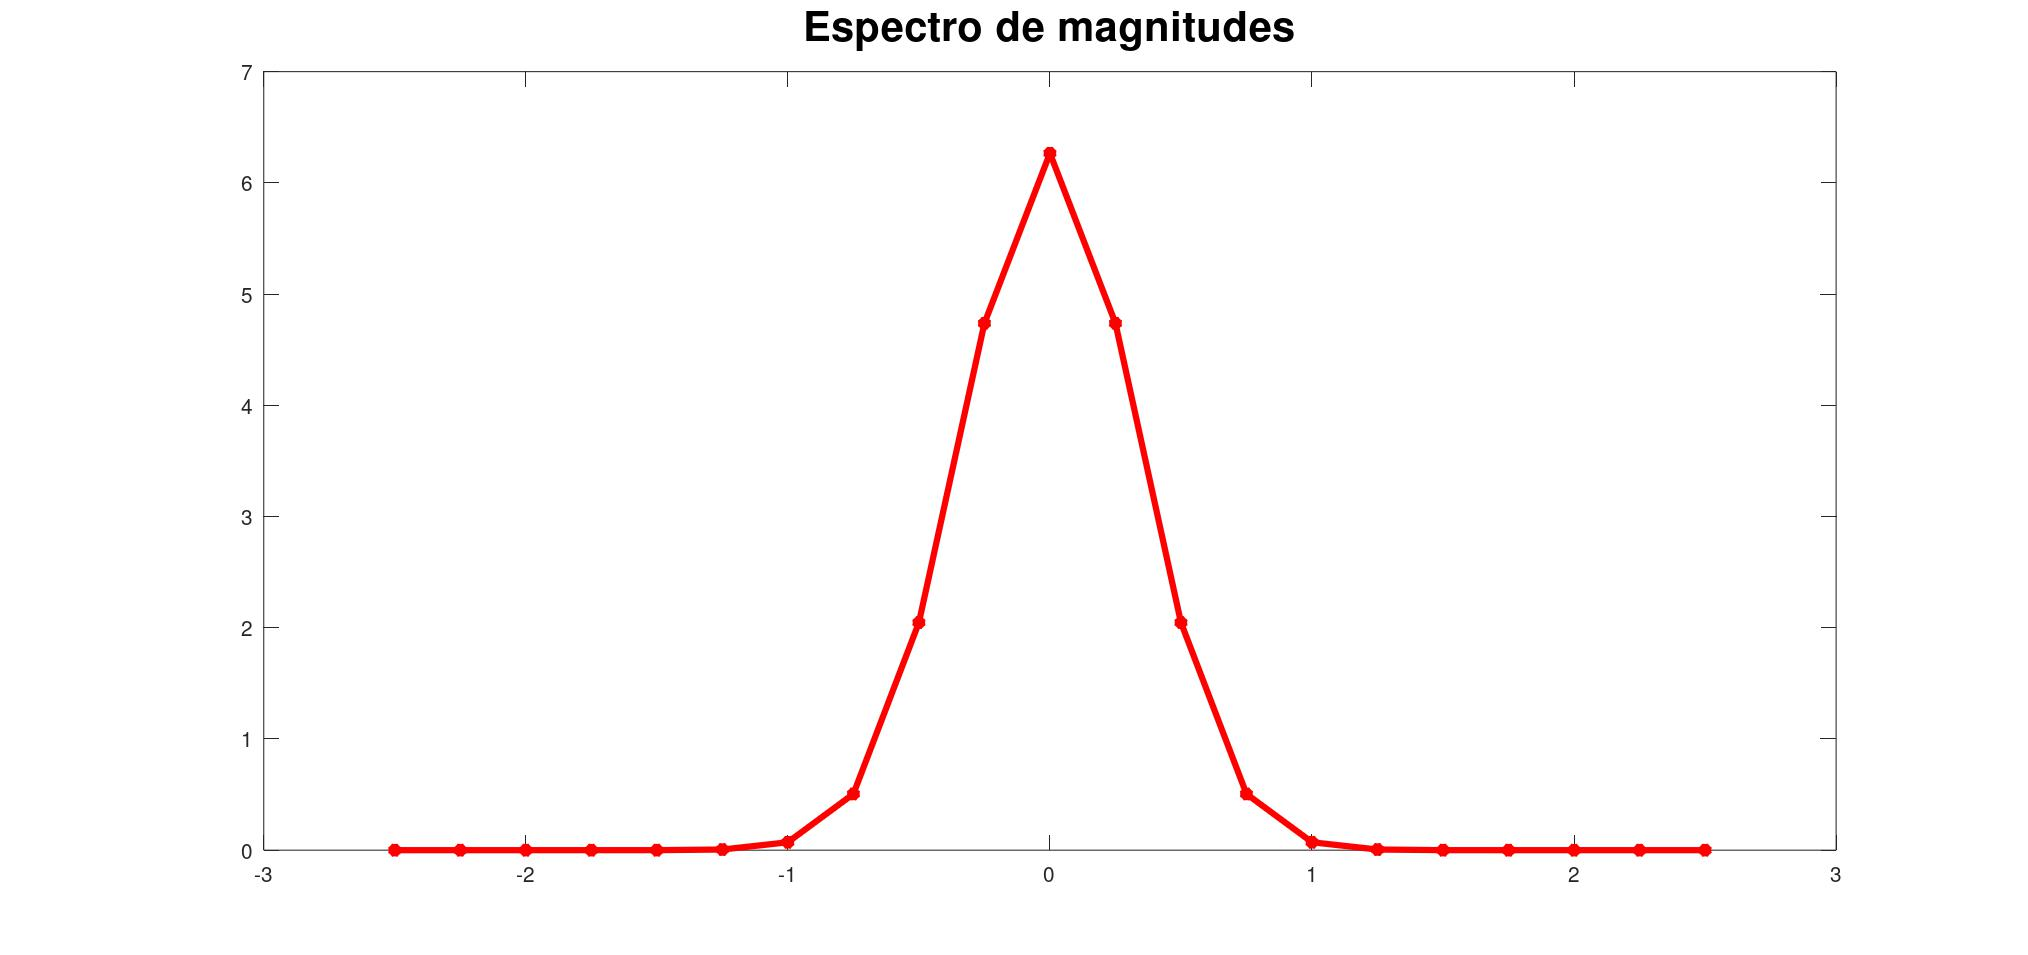
\includegraphics[scale=0.2]{questao1d2}
    \centering
\end{figure}

(e) siga o roteiro acima até não haver diferenças entre significativas entre os espectros;

\vspace{\baselineskip}
Depois de repetir o processo diversas vezes até não ter uma significativa foi obtido o seguinte código final com $\Delta_t$ de 0,0005:

\begin{verbatim}
dt=0.0005;
t=-2:dt:2;
v=exp(-2*t.^2);
f=-(1/(2*dt)):(1/4):(1/(2*dt));
V = fft(v)
V = fftshift(V);
modV = abs(V);
plot(f, modV, "r*")
title("Espectro de magnitudes", "fontsize", 20);    
\end{verbatim}

\begin{figure}[h]
    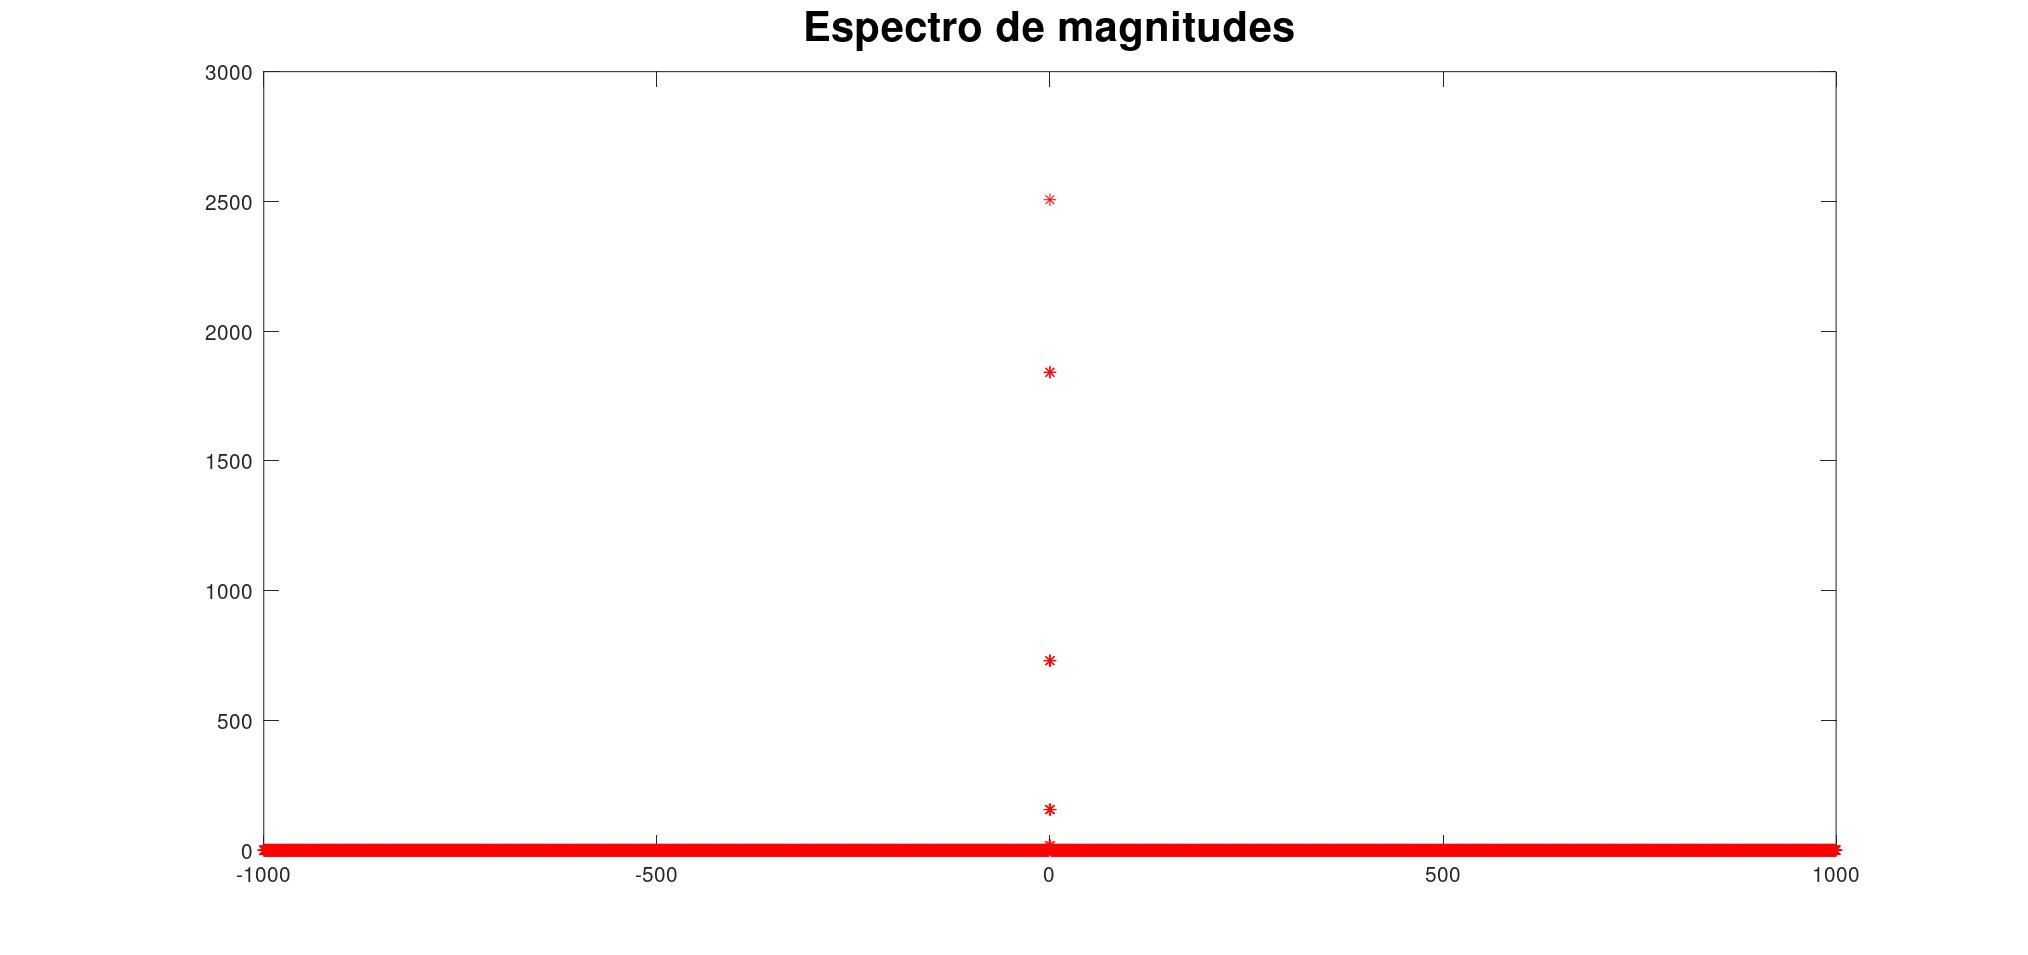
\includegraphics[scale=0.2]{questao1e}
    \centering
\end{figure}

(f) usando esta $f_a$ ''boa'' altere a largura inicial da janela, obtenha o espectro mais uma vez e compare.


\vspace{\baselineskip}


\textbf{2.)} Para o sinal contínuo a seguir (\textbf{Grupo 2:})
\[\text{\textbf{G2: }} x(t) = 8\sinc(4t) - 2\sinc(2t)\]

(a) Plote o gráfico;

\begin{verbatim}
%Questão 2.a)
% Intervalo
dt=0.001;
% Dados basicos
t=-10:dt:10-dt;
x=8*sinc(4*t)-2*sinc(2*t);
plot (t, x, "r", "linewidth", 3);
title("x(t) por t - 2.a)", "fontsize", 20);
xlabel("t", "fontsize", 18);
ylabel("x(t)", "fontsize", 18);
\end{verbatim}

\begin{figure}[h]
    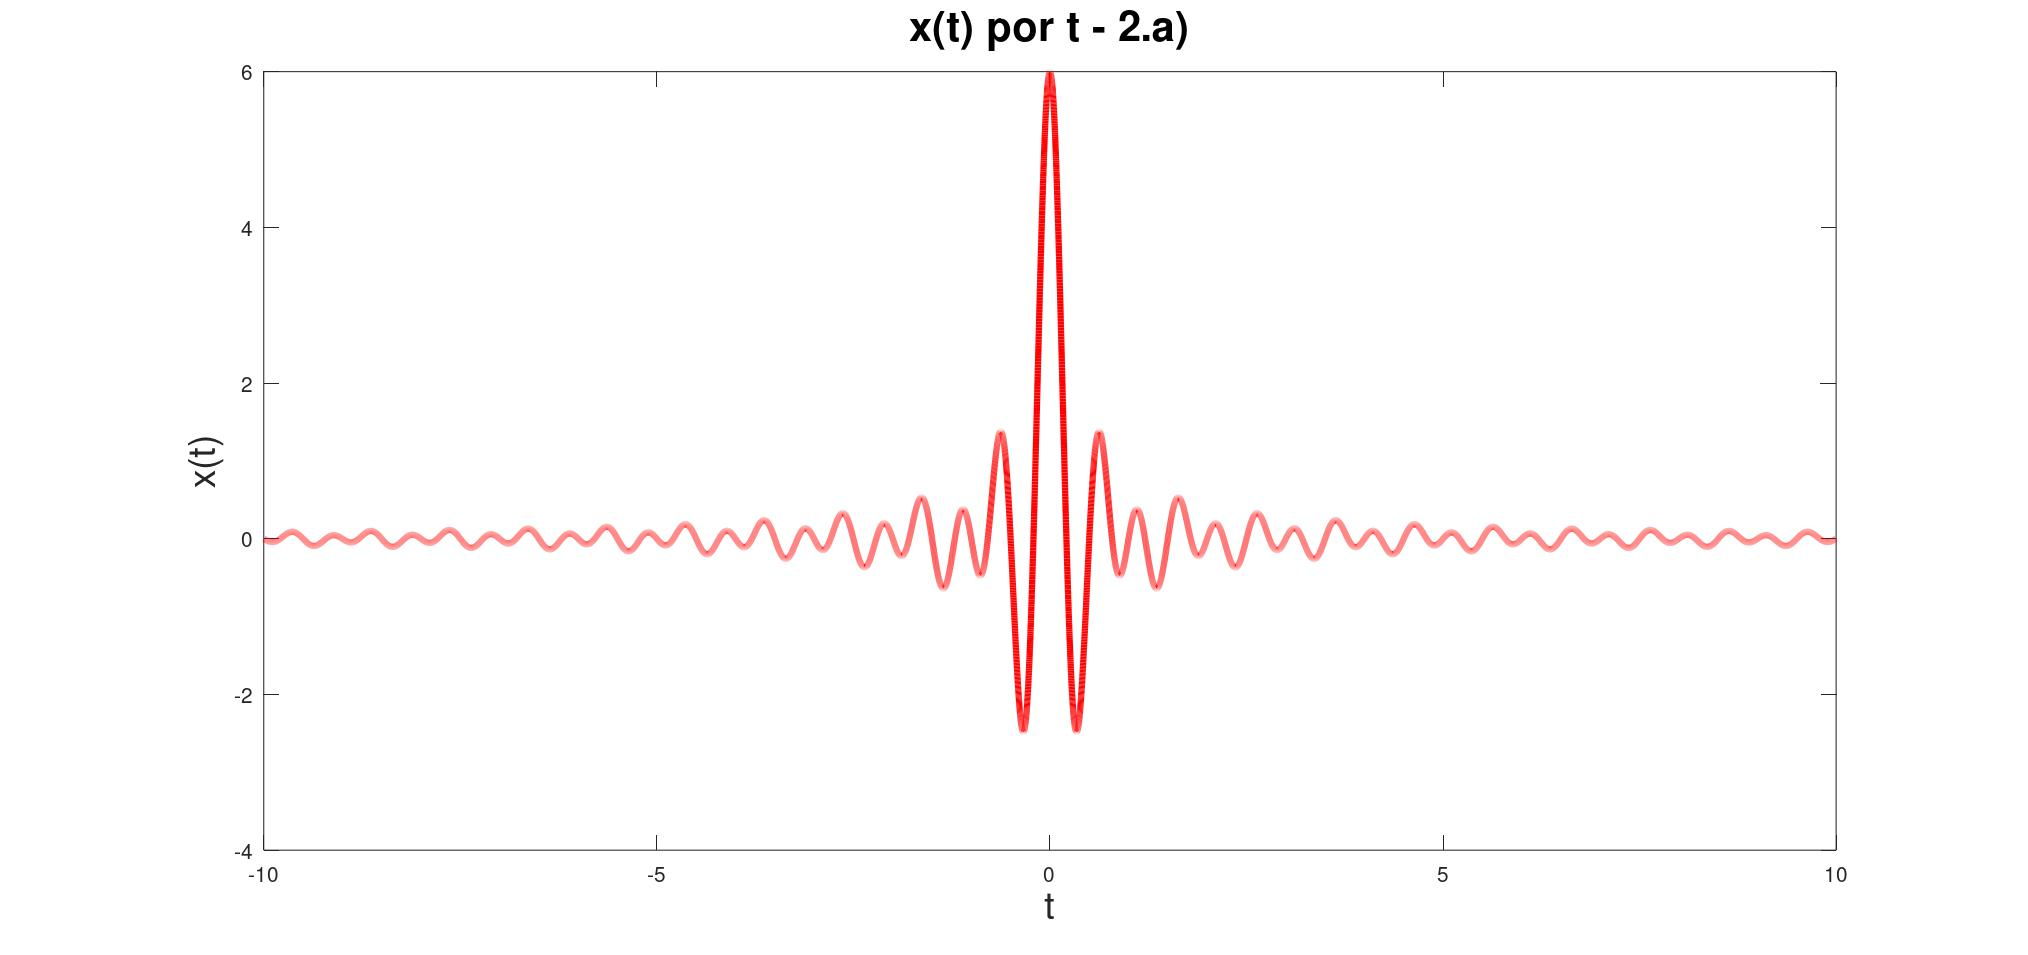
\includegraphics[scale=0.25]{questao2a}
    \centering
\end{figure}

(b) encontre, justificando, a largura $T_0$ de uma janela de observação centrada na origem;

\vspace{\baselineskip}

A largura $T_0$ encontrada foi 8 que começa em -4, porque é o trecho em que maior parte da energia é concentrada e o valor dos máximos e mínimos locais fora desse intervalo deixam de ser tão diferentes.

\vspace{\baselineskip}

(c) idem período de amostragem $\Delta t$ seguro;

(d) encontre o número de pontos $N = 1 + T_0 / (\Delta t)$ e o vetor base de tempo $t = -T_0 / 2 : \Delta t : T_0 / 2$;

(e) construa a escala frequencial $\Delta f = 1 / T_0, F_0 = (N - 1)\Delta f$ e $f = -F_0 / 2 : \Delta f : F_0 / 2$;

(f) encontre os vetores \texttt{x, X = fft(x)} e \texttt{mod = abs(x)};

(g) plote o espectro de amplitude: \texttt{plot(f, mod)};

(h) comente os resultados.


\vspace{\baselineskip}


\textbf{3.)} Os pulsos a seguir são pares e nulos para $\mid t \mid > \Delta$:

$p_{\Delta}$ é o plano $p_{\Delta}(t) = \Delta$ para $\mid t \mid\,\,\leq\,\, \Delta$,

$r_{\Delta}$ é triangular com $r_{\Delta}(-\Delta) = r_{\Delta}(\Delta) = 0$ e $r_{\Delta}(0) = \pi / 2$ e

$c_{\Delta}$ é uma semicircunferência com $c_{\Delta}(-\Delta) = c_{\Delta}(\Delta) = 0$ e $c_{\Delta}(0) = \Delta$.

(a) Esboçar o gráfico para os três pulsos e para (\textbf{Grupo 2:})
\[x = p_4(t) + r_2(t - 2) - c_2(t + 2)\]

(b) Traçar os espectros de x(t), via FFT, determinando $T_0$ e $f_0$ por tentativa e erros.


\vspace{\baselineskip}


\textbf{4.)} Sendo $p_{\tau}(t) = e^{-\Delta (t - \tau)^2}$ uma janela amostradora, com $\Delta = 0.5$ considere os sinais contínuos

\begin{flushleft}
\begin{align*}
    x_1 &= \cos(2 \pi 261.1 t)\\
    x_2 &= \cos(2 \pi 293.7 t)\\
    x_3 &= \cos(2 \pi 311.1 t)\\
    x_4 &= \cos(2 \pi 329.6 t)\\
    x_5 &= \cos(2 \pi 349.2 t)\\
    x_6 &= \cos(2 \pi 392.0 t)\\
    x_7 &= \cos(2 \pi 440.0 t)\\
    x_8 &= \cos(2 \pi 466.2 t)\\
    x_9 &= \cos(2 \pi 522.2 t)
\end{align*}
\end{flushleft}
e as combinações entre eles (\textbf{Grupo 2:})
\[x(t) = x_1p_4 + x_2p_{12} + x_4p_{20} + x_1p_{28} + x_1p_{36} + x_2p_{44} + x_7p_{52} + x_1p_{60} + x_4p_{68} + x_5p_{76} + x_6p_{84}\]

Se estiver usando o MATLAB/Octave use o comando \texttt{sound} ou o \texttt{wavplay} e ouça os sinais $x_i$ e $x$; no FAWAV use o comando \emph{Graph/Audio} com 16 bits, taxa de 8820 e volume de 32000.

(a) Plote o gráfico de $x(t)$ e, a partir dele;

(b) estime a mínima frequência de amostragem $f_a$ segura e uma resolução frequencial $\Delta f$ adequada;

(c) amostre $x$, calcule sua DFT, e plote os espectros com escalas apropriadas;

(d) calcule a energia $E$ do sinal.

(e) Mantendo os pulsos $p_{\tau}$ fixos, construa um sinal $x_a(t)$ fazendo uma permutação aleatória nos ''coeficientes'' $x_i$;

(f) ouça o sinal alterado;

(g) repita (b) e (c) para o novo sinal;

(h) comente os resultados.

\end{document}